\section{How do generative models work? How do GANs compare to others?}
\label{sec:tree}

We now have some idea of what generative models can do and why it might be
desirable to build one.
Now we can ask: how does a generative model actually work? And in particular,
how does a GAN work, in comparison to other generative models?

\subsection{Maximum likelihood estimation}

To simplify the discussion somewhat, we will focus on generative models
that work via the principle of \newterm{maximum likelihood}.
Not every generative model uses maximum likelihood.
Some generative models do not use maximum likelihood by default, but
can be made to do so (GANs fall into this category).
By ignoring those models that do not use maximum likelihood, and
by focusing on the maximum likelihood version of models that do not
usually use maximum likelihood, we can eliminate some of the more 
distracting differences between different models.

The basic idea of maximum likelihood is to define a model that provides
an estimate of a probability distribution, parameterized by parameters
$\vtheta$.
We then refer to the \newterm{likelihood} as the probability that the model
assigns to the training data: $\prod_{i=1}^m \pmodel\left(\vx^{(i)}; \vtheta \right),$
for a dataset containing $m$ training examples $\vx^{(i)}$.

The principle of maximum likelihood simply says to choose the parameters for the model
that maximize the likelihood of the training data.
This is easiest to do in log space, where we have a sum rather than a product
over examples.
This sum simplifies the algebraic expressions for the derivatives of the likelihood
with respect to the models, and when implemented on a digital computer, is less
prone to numerical problems, such as underflow resulting from multiplying together
several very small probabilities.

\begin{align}
\vtheta^* =& \argmax_\vtheta \prod_{i=1}^m \pmodel\left(\vx^{(i)}; \vtheta \right) \\
  =& \argmax_\vtheta \log \prod_{i=1}&m \pmodel\left(\vx^{(i)}; \vtheta \right) \label{eq:log} \\
          =& \argmax_\vtheta \sum_{i=1}^m \log \pmodel\left(\vx^{(i)}; \vtheta \right).
\end{align}

In \eqref{eq:log}, we have used the property that $\argmax_v f(v) = \argmax_v \log f(v)$ for 
positive $v$, because the logarithm is a function that increases everywhere and does not change
the location of the maximum.

The maximum likelihood process is illustrated in \figref{fig:mle}.

We can also think of maximum likelihood estimation as minimizing the
\newterm{KL divergence} between the data generating distribution and the
model:
\[ \vtheta^* = \argmin_\vtheta \KL\left( \pdata(\vx) \Vert \pmodel(\vx ; \vtheta) \right). \]
If we were able to do this precisely, then if $\pdata$ lies within the family of distributions
$\pmodel(\vx ; \vtheta)$, the model would recover $\pdata$ exactly.
In practice, we do not have access to $\pdata$ itself, but only to a training set
consisting of $m$ samples from $\pdata$.
We uses these to define $\ptrain$, an \newterm{empirical distribution} that places mass only
on exactly those $m$ points, approximating $\pdata$.
Minimizing the KL divergence between $\ptrain$ and $\pmodel$ is exactly equivalent to maximizing
the log-likelihood of the training set.

\begin{figure}
\centering
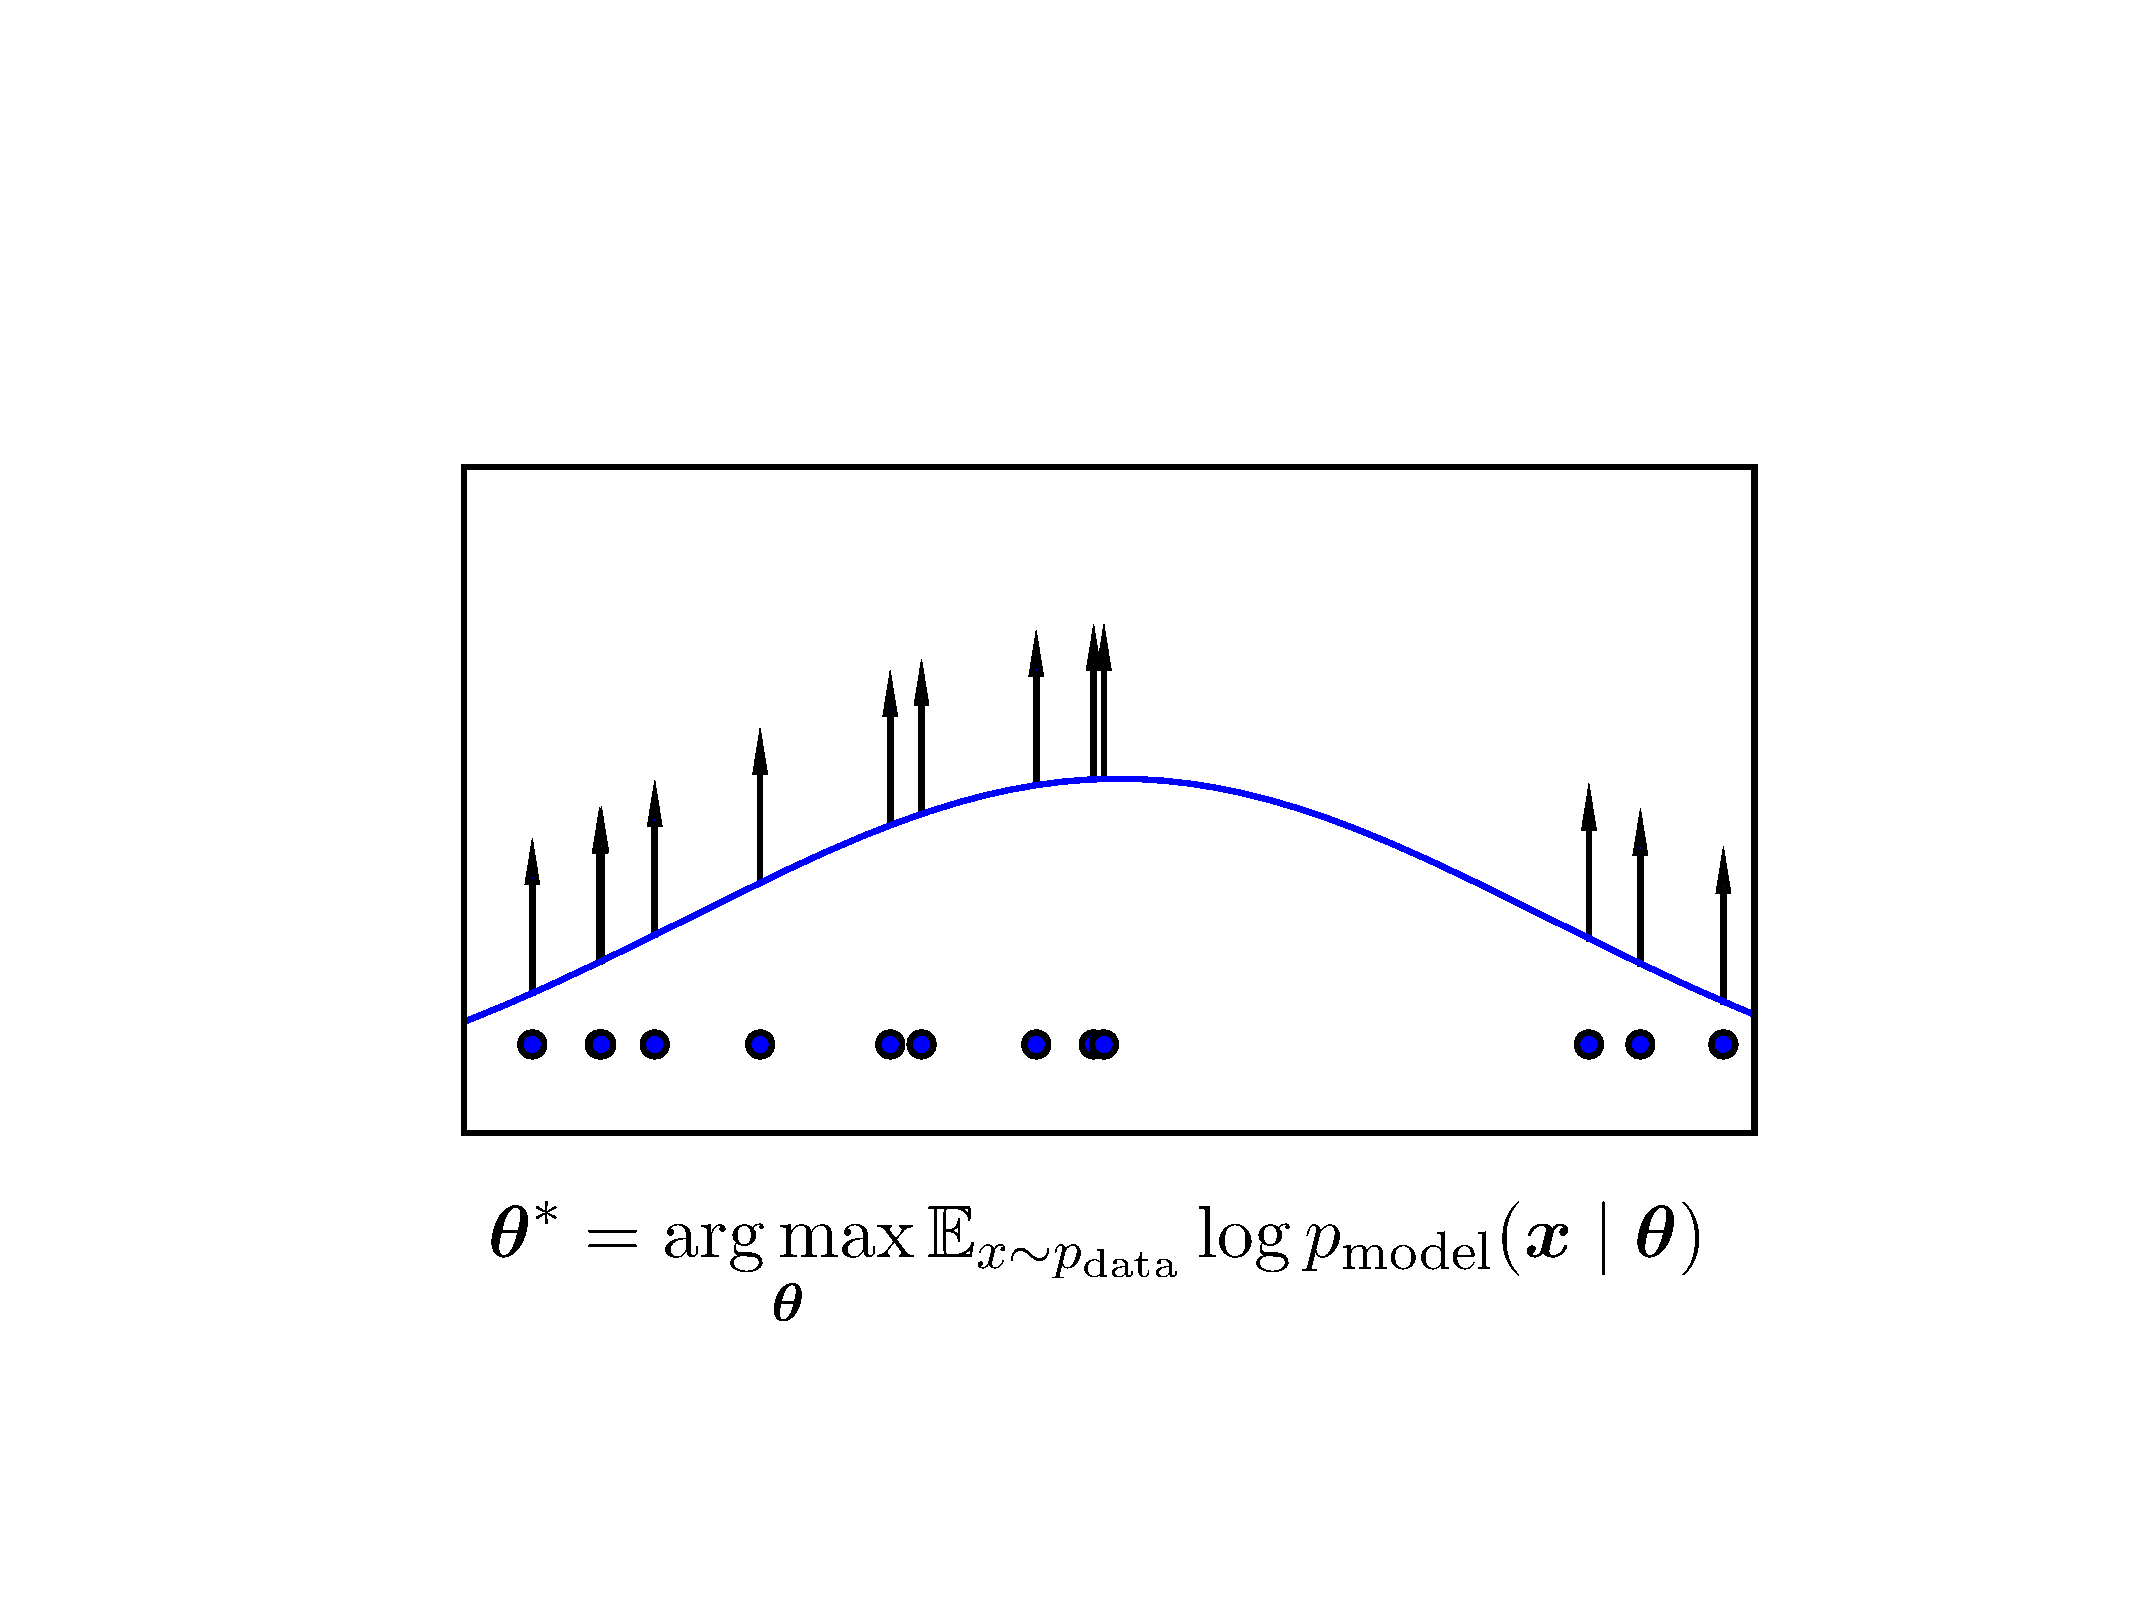
\includegraphics[width=\textwidth]{mle.pdf}
\caption{The maximum likelihood process consists of taking several samples from
  the data generating distribution to form a training set, then pushing up on the
  probability the model assigns to those points, in order to maximize the likelihood
  of the training data.
  This illustration shows how different data points push up on different parts of
  the density function for a Gaussian model applied to 1-D data.
  The fact that the density function must sum to $1$ means that we cannot simply
  assign infinite likelihood to all points; as one point pushes up in one place
  it inevitably pulls down in other places.
  The resulting density function balances out the upward forces from all the data
  points in different locations.
}
\label{fig:mle}
\end{figure}

For more information on maximum likelihood and other statistical estimators,
see chapter 5 of \citet{Goodfellow-et-al-2016}.


\subsection{A taxonomy of deep generative models}

If we restrict our attention to deep generative models that work by maximizing
the likelihood, we can compare several models by contrasting the ways that they
compute either the likelihood and its gradients, or approximations to these
quantities.
As mentioned earlier, many of these models are often used with principles other
than maximum likelihood, but we can examine the maximum likelihood variant of
each of them in order to reduce the amount of distracting differences between
the methods.
Following this approach, we construct the taxonomy shown in \figref{fig:tree}.
Every leaf in this taxonomic tree has some advantages and disadvantages.
GANs were designed to avoid many of the disadvantages present in pre-existing
nodes of the tree, but also introduced some new disadvantages.

\begin{figure}
\centering
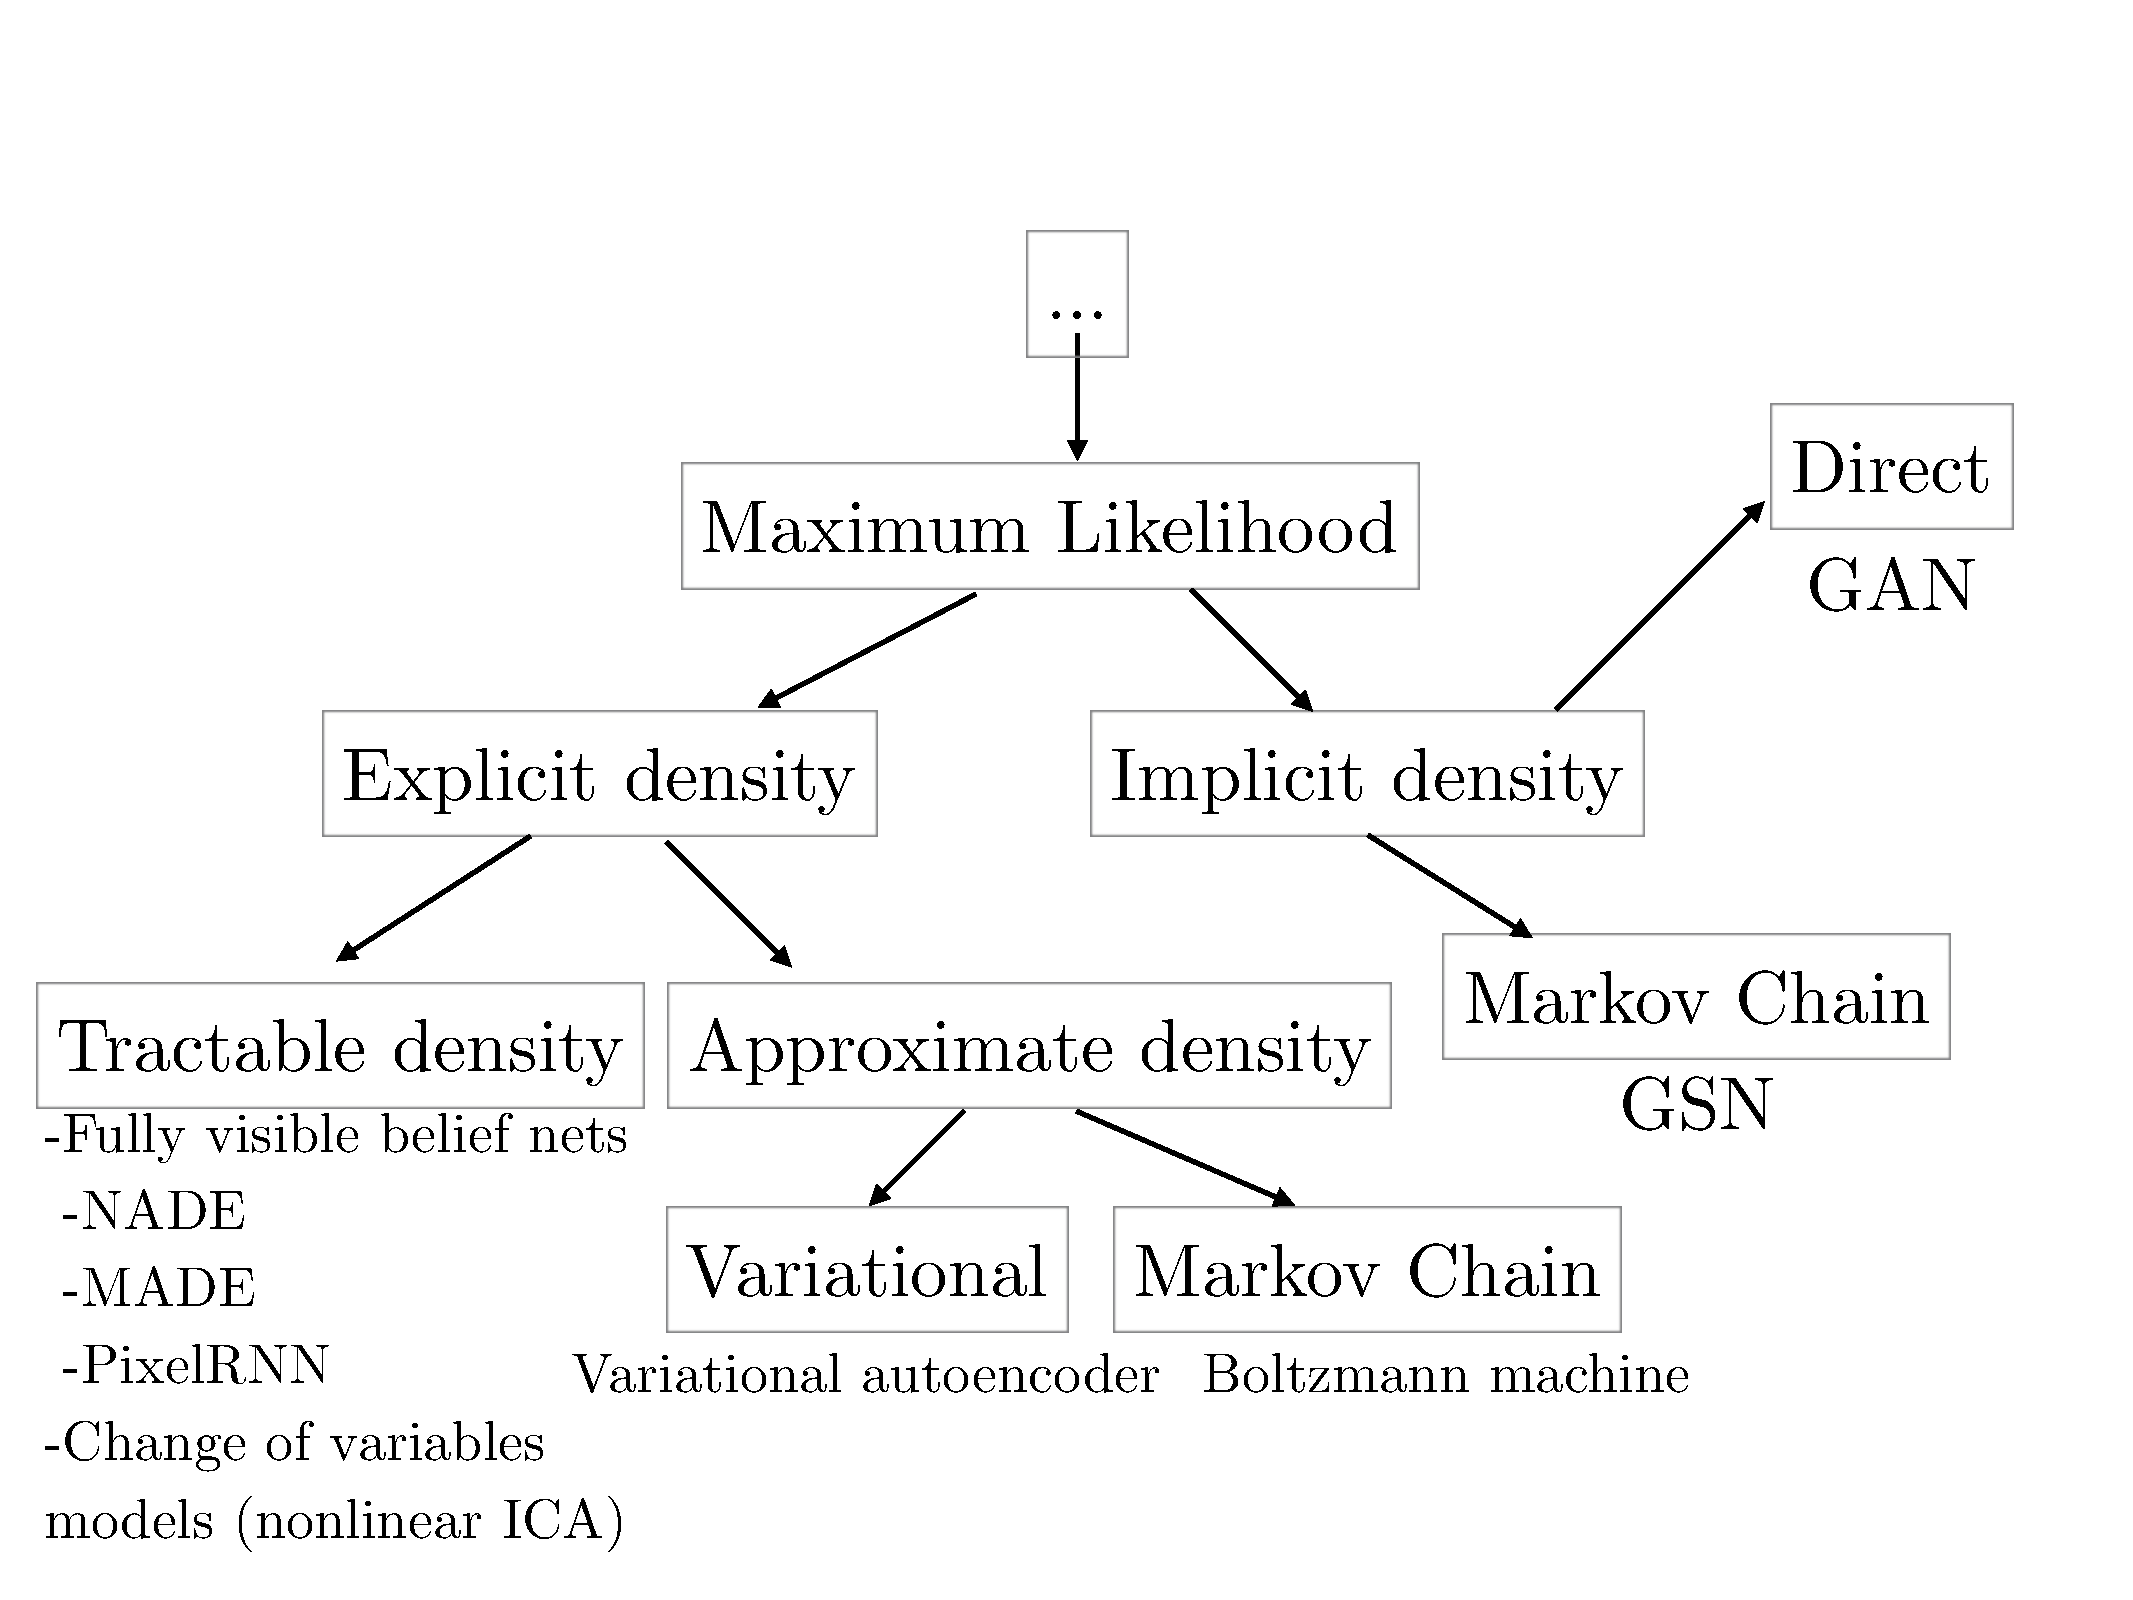
\includegraphics[width=\textwidth]{tree}
\caption{
Deep generative models that can learn via the principle of maximim likelihood
differ with respect to how they represent or approximate the likelihood.
On the left branch of this taxonomic tree, models construct an explicit density,
$\pmodel(\vx; \vtheta)$, and thus an explicit likelihood which can be maximized.
Among these explicit density models, the density may be computationally tractable,
or it may be intractable, meaning that to maximize the likelihood it is necessary
to make either variatioanl approximations or Monte
Carlo approximations (or both).
On the right branch of the tree, the model does not explicitly represent a
probability distribution over the space where the data lies.
Instead, the model provides some way of interacting less directly with this
probability distribution.
Typically the indirect means of interacting with the probability distribution is
the ability to draw samples from it.
Some of these implicit models that offer the ability to sample from the distribution
do so using a Markov Chain; the model defines a way to stochastically transform
an existing sample in order to obtain another sample from the same distribution.
Others are able to generate a sample in a single step, starting without any input.
While the models used for GANs can sometimes be constructed to define an explicit
density, the training algorithm for GANs makes use only of the model's ability to
generate samples.
GANs are thus trained using the strategy from the rightmost leaf of the tree:
using an implicit model that samples directly from the distribution represented
by the model.
}
\label{fig:tree}
\end{figure}

\subsection{Explicit density models}

In the left branch of the taxonomy shown in \figref{fig:tree} are models that define
an explicit density function $\pmodel(\vx ; \vtheta)$.
For these models, maxmimization of the likelihood is straightforward; we simply plug
the model's definition of the density function into the expression for the likelihood,
and follow the gradient uphill.

The main difficulty present in explicit density models is designing a model that can
capture all of the complexity of the data to be generated 
while still maintaining computational tractability.
There are two different strategies used to confront this challenge:
(1) careful construction of models whose structure guarantees their tractability,
as described in \secref{sec:explicit_tractable},
and (2) models that admit tractable approximations to the likelihood and its
gradients, as described in \secref{sec:approx}.

\subsubsection{Tractable explicit models}
\label{sec:explicit_tractable}

In the leftmost leaf of the taxonomic tree of \figref{fig:tree} are the models
that define an explicit density function that is computationally tractable.
There are currently two popular approaches to tractable explicit density models:
fully visible belief networks and nonlinear independent components analysis.

\paragraph{Fully visible belief networks}
\newterm{Fully visible belief networks} \citep{Frey96,Frey98} or FVBNs are models that use the chain
rule of probability to decompose a probability distribution over an $n$-dimensional vector $\vx$
into a product of one-dimensional probability distributions:
\[
\pmodel(\vx) = \prod_{i=1}^n \pmodel\left(\evx_i \mid \evx_1, \dots, \evx_{i-1} \right).
\]
FVBNs are, as of this writing, one of the three most popular
approaches to generative modeling, alongside GANs and variational autoencoders.
They form the basis for sophisticated generative models from DeepMind, such as
WaveNet \citep{aaron-wavenet-2016}. WaveNet is able to generate realistic human speech.
The main drawback of FVBNs is that samples must be generated
one entry at a time: first $\evx_1$, then $\evx_2$, etc., so the cost of generating
a sample is $O(n)$.
In modern FVBNs such as WaveNet, the distribution over each $\evx_i$ is computed by a deep
neural network, so each of these $n$ steps involves a nontrivial amount of computation.
Moreover, these steps cannot be parallelized.
WaveNet thus requires two minutes of computation time to generate one second of audio,
and cannot yet be used for interactive conversations.
GANs were designed to be able to generate all of $\vx$ in parallel, yielding greater
generation speed.

\paragraph{Nonlinear independent components analysis}
Another family of deep generative models with explicit density functions is based on
defining continuous, nonlinear transformations between two different spaces.
For example, if there is a vector of latent variables $\vz$ and a continuous, differentiable,
invertible transformation
$g$ such that $g(\vz)$ yields a sample from the model in $\vx$ space,
then
\begin{equation}
  \label{eq:change-of-variable}
  p_x(\vx) = p_z(g^{-1}(\vx)) \left| \mathrm{det}
  \left( \frac{\partial g^{-1}(\vx)} {\partial \vx}\right) \right|. 
\end{equation}
The density $p_x$ is tractable if the density $p_z$ is tractable
and the determinant of the Jacobian of $g^{-1}$ is tractable.
In other words, a simple distribution over $\vz$ combined with
a transformation $g$ that warps space in complicated ways can yield
a complicated distribution over $\vx$, and if $g$ is carefully designed,
the density is tractable too.
Models with nonlinear $g$ functions date back at least to
~\citet{hyvarinen1999nonlinear}.
The latest member of this family is real NVP \citep{dinh2016density}.
See \figref{fig:nvp} for some visualizations of ImageNet samples
generated by real NVP.
The main drawback to nonlinear ICA models is that they impose restrictions
on the choice of the function $g$. In particular, the invertibility requirement
means that the latent variables $\vz$ must have the same dimensionality as $\vx$.
GANs were designed to impose very few requirements on $g$, and, in particular,
admit the use of $\vz$ with larger dimension than $\vx$.

\begin{figure}
\centering
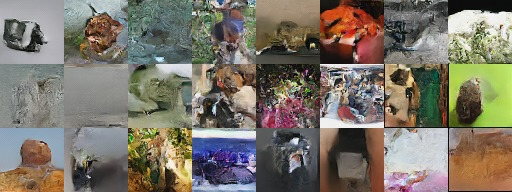
\includegraphics[width=\textwidth]{fig_imnet_64_samples}
\caption{Samples generated by a real NVP model trained on 64x64 ImageNet images.
Figure reproduced from \citet{dinh2016density}.}
\label{fig:nvp}
\end{figure}

For more information about the chain rule of probability used to define FVBNs
or about the effect of deterministic transformations on probability densities
as used to define nonlinear ICA models, see chapter 3 of \citet{Goodfellow-et-al-2016}.

In summary, models that define an explicit, tractable density are highly
effective, because they permit the use of an optimization algorithm directly
on the log-likelihood of the training data.
However, the family of models that provide a tractable density is limited,
with different families having different disadvantages.

\subsubsection{Explicit models requiring approximation}
\label{sec:approx}

To avoid some of the disadvantages imposed by the design requirements of models
with tractable density functions, other models have been developed that still
provide an explicit density function but use one that is intractable, requiring
the use of approximations to maximize the likelihood.
These fall roughly into two categories: those using deterministic approximations,
which almost always means variational methods, and those using stochastic approximations,
meaning Markov chain Monte Carlo methods.

\paragraph{Variational approximations}
Variational methods define a lower bound
\[ \mathcal{L}(\vx; \vtheta) \leq \log \pmodel(\vx; \vtheta). \]
A learning algorithm that maximizes $\mathcal{L}$ is guaranteed to obtain at least
as high a value of the log-likelihood as it does of $\mathcal{L}$.
For many families of models, it is possible to define an $\mathcal{L}$ that is computationally
tractable even when the log-likelihood is not.
Currently, the most popular approach to variational learning in deep generative models
is the \newterm{variational autoencoder} \citep{Kingma-arxiv2013,Rezende-et-al-ICML2014} or VAE.
Variational autoencoders are one of the three approaches to deep generative modeling that are
the most popular as of this writing, along with FVBNs and GANs.
The main drawback of variational methods is that the deterministic approximation induces some bias,
in the sense that even with a perfect optimization algorithm and infinite training data, the gap
between $\mathcal{L}$ and the true likelihood can result in $\pmodel$ learning something other than
the true $\pdata$.
GANs were designed to be unbiased, in the sense that with a large enough model and infinite data,
the Nash equilibrium for a GAN game corresponds to recovering $\pdata$ exactly.
In practice, variational methods often obtain very good likelihood, but are regarded as producing
lower quality samples.
There is not a good method of quantitatively measuring sample quality, so this is a subjective opinion,
not an empirical fact.
See \figref{fig:vae_samples} for an example of some samples drawn from a VAE.
While it is difficult to point to a single aspect of GAN design and say that it results in
better sample quality, GANs are generally regarded as producing better samples.
For more information about variational approximations, see chapter 19 of
\citet{Goodfellow-et-al-2016}.

\begin{figure}
  \centering
  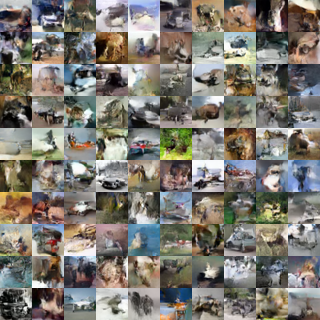
\includegraphics[width=\textwidth]{cifar_vae}
  \caption{Samples drawn from a VAE trained on the CIFAR-10 dataset.
    Figure reproduced from \citet{kingma2016improving}.
  }
  \label{fig:vae_samples}
\end{figure}

\paragraph{Markov chain approximations}
Most deep learning algorithms make use of some form of stochastic approximation,
at the very least in the form of using a small number of randomly selected training
examples to form a minibatch used to minimize the expected loss.
Usually, sampling-based approximations work reasonably well as long as a fair sample
can be generated quickly (e.g. selecting a single example from the training set
is a cheap operation) and as long as the variance across samples is not too high.
Some models require the generation of more expensive samples, using Markov chain
techniques.
A Markov chain is a process for generating samples by repeatedly drawing a sample
$\vx' \sim q(\vx' \mid \vx).$
By repeatedly updating $\vx$ according to the transition operator $q$, Markov chain
methods can sometimes guarantee that $\vx$ will eventually converge to a sample from
$\pmodel(\vx)$.
Unfortunately, this convergence can be very slow, and there is no clear way to test
whether the chain has converged, so in practice one often uses $\vx$ too early, before
it has truly converged to be a fair sample from $\pmodel$.
In high-dimensional spaces, Markov chains become less efficient.
Boltzmann machines \citep{Fahlman83,Ackley85,Hinton-Boltzmann,Hinton86a} are a
family of generative models that rely on Markov chains both to train the model
or to generate a sample from the model.
Boltzmann machines were an important part of the deep learning renaissance beginning
in 2006 \citep{Hinton06,hinton2007learning} but they are now used only very rarely,
presumably mostly because the underlying Markov chain approximation techniques have
not scaled to problems like ImageNet generation.
Moreover, even if Markov chain methods scaled well enough to be used for training,
the use of a Markov chain to generate samples from a trained model is undesirable
compared to single-step generation methods because the multi-step Markov chain
approach has higher computational cost.
GANs were designed to avoid using Markov chains for these reasons.
For more information about Markov chain Monte Carlo approximations, see chapter 18 of
\citet{Goodfellow-et-al-2016}.
For more information about Boltzmann machines, see chapter 20 of the same book.

Some models use both variational and Markov chain approximations.
For example, deep Boltzmann machines make use of both types of
approximation \citep{SalHinton09}.

\subsection{Implicit density models}

Some models can be trained without even needing to explicitly define a density
functions.
These models instead offer a way to train the model while interacting only
indirectly with $\pmodel$, usually by sampling from it.
These constitute the second branch, on the right side, of our taxonomy of
generative models depicted in \figref{fig:tree}.

Some of these implicit models based on drawing samples from $\pmodel$ define
a Markov chain transition operator that must be run several times to obtain
 a sample from the model.
From this family, the primary example is the \newterm{generative stochastic network}
\citep{Bengio-et-al-ICML-2014}.
As discussed in \secref{sec:approx}, Markov chains often fail to scale to high
dimensional spaces, and impose increased computational costs for using the
generative model. GANs were designed to avoid these problems.

Finally, the rightmost leaf of our taxonomic tree is the family of implicit models
that can generate a sample in a single step.
At the time of their introduction, GANs were the only notable member of this family,
but since then they have been joined by additional models based on
kernelized moment matching \citep{Li-et-al-2015,dziugaite2015training}.

\subsection{Comparing GANs to other generative models}

In summary, GANs were designed to avoid many disadvantages associated with other generative
models:
\begin{itemize}
  \item They can generate samples in parallel, instead of using runtime proportional to the
    dimensionality of $\vx$. This is an advantage relative to FVBNs.
  \item The design of the generator function has very few restrictions. This is an advantage
    relative to Boltzmann machines, for which few probability distributions admit tractable
    Markov chain sampling, and relative to nonlinear ICA, for which the generator must be
    invertible and the latent code $\vz$ must have the same dimension as the samples
    $\vx$.
  \item No Markov chains are needed. This is an advantage relative to Boltzmann machines and GSNs.
  \item No variational bound is needed, and thus the GAN framework is able to be asymptotically
    consistent. This is an advantage relative to VAEs.
  \item GANs are subjectively regarded as producing better samples than other methods.
\end{itemize}
